\documentclass{report}

\input{preamble}
\input{macros}
\input{letterfonts}

\title{\Huge{Math 244}}
\author{\huge{PSET 1}}
\date{JAN 24 2025}

\begin{document}

\maketitle
\newpage% or \cleardoublepage
% \pdfbookmark[<level>]{<title>}{<dest>}
\pdfbookmark[section]{\contentsname}{toc}
\tableofcontents
\pagebreak

\section*{Section 1.2 Problem 5}
\addcontentsline{toc}{section}{Problem 1}

\qs{Section 1.2 Problem 5}{
    Is a "cancellation" possible for the Cartesion Product? That is,
    if $X \times Y = X \times Z$ holds for some sets, $X$, $Y$, and $Z$, does it follow that $Y = Z$? 
}

\begin{RemarkWithLily}{What is the Cartesian Product?}
    TThe Cartesian product of $X$ and $Y$ is the set of all ordered pairs of the form $(x,y)$, where $x \in X$ and $y \in Y$. 
\end{RemarkWithLily}

\begin{RemarkWithLily}{Asnwer}
    TThe "cancellation" is not possible for the Cartesian Product unless it is stated that $X$ is not an empty set. For if $X$ is an empty set, then the Cartesian Product of $X$ and 
    another set would always be the empty set. In this scenario, $Y$ and $Z$ could be different and their Cartesian Products with $X$ would still be the empty set.
\end{RemarkWithLily}

\section*{Section 1.2 Problem 6}
\addcontentsline{toc}{section}{Problem 2}

\qs{Section 1.2 Problem 6}{
    Prove that for any two sets $A$, $B$ we have 
    \begin{center}
        \[ \left(A \setminus B\right) \cup \left(B \setminus A \right) = \left( A \cup B \right) \setminus \left( A \cap B \right)\] 
    \end{center}
}

\begin{center}
    \begin{minipage}{0.45\textwidth}
      \centering
      {\footnotesize $A \setminus B$}\\[5pt]
      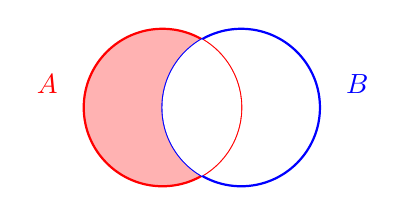
\begin{tikzpicture}[scale=0.5]
        % First Venn Diagram
        \begin{scope}[shift={(0,0)}]
          % Circle A
          \filldraw[
            line width=0.8pt,
            color=red,
            fill=red!30
          ] (0,0) circle[radius=2cm]
            node[left=1.2cm, yshift=0.3cm] {$ A $};
  
          % Circle B
          \filldraw[
            line width=0.8pt,
            color=blue,
            fill=none
          ] (2,0) circle[radius=2cm]
            node[right=1.2cm, yshift=0.3cm] {$ B $};
  
          % Overlap
          \begin{scope}
            \clip (2,0) circle [radius=2cm];
            \fill[white] (0,0) circle [radius=2cm];
          \end{scope}
        \end{scope}
      \end{tikzpicture}
    \end{minipage}
    \hfill
    \begin{minipage}{0.45\textwidth}
      \centering
      {\footnotesize $B \setminus A$}\\[5pt]
      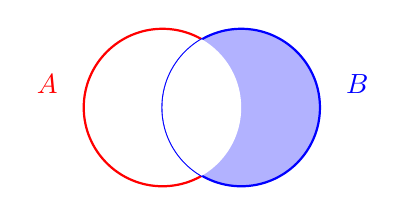
\begin{tikzpicture}[scale=0.5]
        % Second Venn Diagram
        \begin{scope}[shift={(0,0)}]
          % Circle A
          \filldraw[
            line width=0.8pt,
            color=red,
            fill=none
          ] (0,0) circle[radius=2cm]
            node[left=1.2cm, yshift=0.3cm] {$ A $};
  
          % Circle B
          \filldraw[
            line width=0.8pt,
            color=blue,
            fill=blue!30
          ] (2,0) circle[radius=2cm]
            node[right=1.2cm, yshift=0.3cm] {$ B $};
  
          % Overlap
          \begin{scope}
            \clip (0,0) circle [radius=2cm];
            \fill[white] (2,0) circle [radius=2cm];
          \end{scope}
        \end{scope}
      \end{tikzpicture}
    \end{minipage}
\end{center}  

\begin{center}
    {\footnotesize $(A \setminus B) \cup (B \setminus A)$}\\[5pt]
    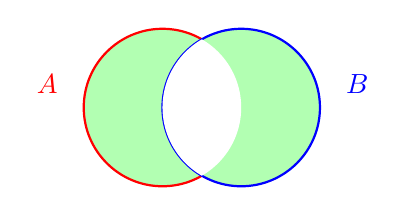
\begin{tikzpicture}[scale=0.5]
        % Circle A
        \filldraw[
          line width=0.8pt,
          color=red,
          fill=green!30
        ] (0,0) circle[radius=2cm]
          node[left=1.2 cm, yshift=0.3cm] {$ A $};
        
        % Circle B
        \filldraw[
          line width=0.8pt,
          color=blue,
          fill=green!30
        ] (2,0) circle[radius=2cm]
          node[right=1.2 cm, yshift=0.3cm] {$ B $};
    
        % Overlap
        \begin{scope}
          \clip (0,0) circle [radius=2cm]; 
          \fill[white] (2,0) circle [radius=2cm]; 
        \end{scope}
    \end{tikzpicture}
\end{center}
  
\begin{center}
    \begin{minipage}{0.45\textwidth}
      \centering
      {\footnotesize $A \cup B $}\\[5pt]
      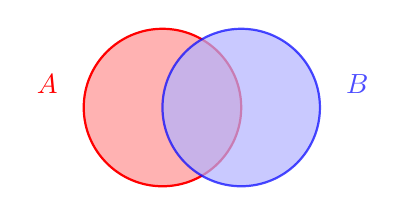
\begin{tikzpicture}[scale=0.5]
        \begin{scope}[shift={(-4,0)}]
          % Circle A
          \filldraw[
            line width=0.8pt,
            color=red,
            fill=red!30,
            draw=red
          ] (0,0) circle[radius=2cm]
            node[left=1.2cm, yshift=0.3cm] {$ A $};
          
          % Circle B with transparency
          \filldraw[
            line width=0.8pt,
            color=blue,
            fill=blue!30,
            draw=blue,
            opacity=0.7
          ] (2,0) circle[radius=2cm]
            node[right=1.2cm, yshift=0.3cm] {$ B $};
        \end{scope}
      \end{tikzpicture}
    \end{minipage}
    \hfill
    \begin{minipage}{0.45\textwidth}
      \centering
      {\footnotesize $A \cap B$ }\\[5pt]
      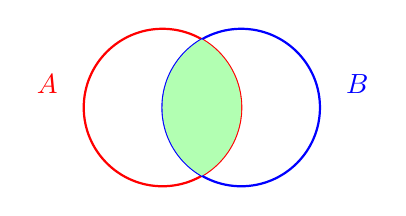
\begin{tikzpicture}[scale=0.5]
        \begin{scope}[shift={(5,0)}]
          % Circle A
          \filldraw[
            line width=0.8pt,
            color=red,
            fill=none
          ] (0,0) circle[radius=2cm]
            node[left=1.2cm, yshift=0.3cm] {$ A $};
          
          % Circle B
          \filldraw[
            line width=0.8pt,
            color=blue,
            fill=none
          ] (2,0) circle[radius=2cm]
            node[right=1.2cm, yshift=0.3cm] {$ B $};
          
          % Overlap
          \begin{scope}
            \clip (0,0) circle [radius=2cm]; 
            \fill[green!30] (2,0) circle [radius=2cm]; 
          \end{scope}
        \end{scope}
      \end{tikzpicture}
    \end{minipage}
\end{center}
  
\begin{center}
    {\footnotesize $(A \cup B) \setminus (A \cap B)$}\\[5pt]
    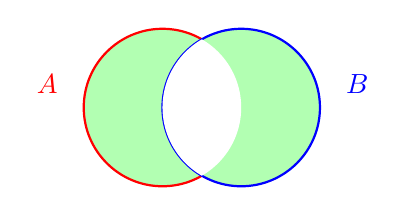
\begin{tikzpicture}[scale=0.5]
        % Circle A
        \filldraw[
          line width=0.8pt,
          color=red,
          fill=green!30
        ] (0,0) circle[radius=2cm]
          node[left=1.2cm, yshift=0.3cm] {$ A $};
        
        % Circle B
        \filldraw[
          line width=0.8pt,
          color=blue,
          fill=green!30
        ] (2,0) circle[radius=2cm]
          node[right=1.2cm, yshift=0.3cm] {$ B $};
    
        % Overlap
        \begin{scope}
          \clip (0,0) circle [radius=2cm]; 
          \fill[white] (2,0) circle [radius=2cm]; 
        \end{scope}
    \end{tikzpicture}
\end{center}
  
\begin{ClaimWithMagnolia}{Claim 1 For Probelm 2}
    IIf $x \in \left(A \setminus B\right) \cup \left(B \setminus A \right)$, then $x \in A \setminus B$ or $x \in B \setminus A$.
\end{ClaimWithMagnolia}

\begin{RemarkWithLily}{1}
    IIf $x \in A \setminus B$, then $x \in A$ and $x \notin B$. This also implies $x \in A \cup B$ but $x \notin A \cap B$, so $x \in (A \cup B) \setminus (A \cap B)$. \\
    If $x \in B \setminus A$, then $x \in B$ and $x \notin A$, which implies $x \in A \cup B$ but $x \notin A \cap B$, so $x \in (A \cup B) \setminus (A \cap B)$. \\
    
    This proves that:
    \[
    \left(A \setminus B\right) \cup \left(B \setminus A \right) \subseteq \left( A \cup B \right) \setminus \left( A \cap B \right).
    \]
\end{RemarkWithLily}

\begin{ClaimWithMagnolia}{Claim 2 For Probelm 2}
    IIf $x$ is in $\left( A \cup B \right) \setminus \left( A \cap B \right)$, then $x \in A \cup B$ and $x \notin A \cap B$.
\end{ClaimWithMagnolia}

\begin{RemarkWithLily}{2}
    IIf $x \in A \cup B$ but $x \notin A \cap B$, then $x$ must belong to exactly one of $A$ or $B$. \\
    If $x \in A$ but $x \notin B$, then $x \in A \setminus B$. \\
    If $x \in B$ but $x \notin A$, then $x \in B \setminus A$. \\
    
    Therefore, $x \in \left(A \setminus B\right) \cup \left(B \setminus A \right)$.

    This proves that:
    \[
    \left( A \cup B \right) \setminus \left( A \cap B \right) \subseteq \left(A \setminus B\right) \cup \left(B \setminus A \right).
    \]
\end{RemarkWithLily}


\section*{Section 1.3 Problem 2}
\addcontentsline{toc}{section}{Problem 3}

\qs{Section 1.3 Problem 2}{
    The numbers $F_{0}$, $F_{1}$, $F_{2}$, $F_{3}$, $\ldots$ are defined as follows:
        \begin{center}
            \[ F_{0} = 0, F_{1} = 1, F_{n+2} = F_{n+1} + F_{n} \text{for } n = 0,1,2, \ldots \] 
        \end{center}
    Prove that for any $n \geq 0$ we have $F_{n} \leq \left(\frac{1 + \sqrt{5}}{2}\right)^{n-1}$
}

\begin{basecaseWithPoppy}
    The formula $F_{n} \leq \left(\frac{1 + \sqrt{5}}{2}\right)^{n-1}$ holds for $ n = 0 $ since $ F_{0} = 0 $ and $ \left(\frac{1 + \sqrt{5}}{2}\right)^{-1} = \frac{2}{1 + \sqrt{5}} $.  \\
    The formula $F_{n} \leq \left(\frac{1 + \sqrt{5}}{2}\right)^{n-1}$ holds for $ n = 1 $ since $ F_{1} = 1 $ and $ \left(\frac{1 + \sqrt{5}}{2}\right)^{0} = 1 $. 
\end{basecaseWithPoppy}

\begin{inducthypWithRose}
  Let us suppose that the formula $F_{n} \leq \left(\frac{1 + \sqrt{5}}{2}\right)^{n-1}$ and $F_{n+1} \leq \left(\frac{1 + \sqrt{5}}{2}\right)^{n}$ holds for some $n \geq 0$.
\end{inducthypWithRose}  

\begin{RemarkWithLily}{The Golden Ratio}
   H$\phi$ is equal to $\frac{1 + \sqrt{5}}{2}$.    
\end{RemarkWithLily}

\begin{inductstepWithTulip}
  Using the Fibonacci recurrence relation $F_{n+2} = F_{n+1} + F_{n}$ and the inductive hypothesis:
  \[ F_{n+2} \leq \left(\frac{1 + \sqrt{5}}{2}\right)^{n} + \left(\frac{1 + \sqrt{5}}{2}\right)^{n-1}. \]
  Factor out $\left(\frac{1 + \sqrt{5}}{2}\right)^{n-1}$:
  \[ F_{n+2} \leq \left(\frac{1 + \sqrt{5}}{2}\right)^{n-1} \left( \frac{1 + \sqrt{5}}{2} + 1 \right). \]
  Since $\frac{1 + \sqrt{5}}{2} + 1 = \frac{3 + \sqrt{5}}{2} = \left(\frac{1 + \sqrt{5}}{2}\right)^2$, we have:
  \[ F_{n+2} \leq \left(\frac{1 + \sqrt{5}}{2}\right)^{n-1} \cdot \left(\frac{1 + \sqrt{5}}{2}\right)^2 = \left(\frac{1 + \sqrt{5}}{2}\right)^{n+1}. \]
  $\therefore \forall n \geq 0$ 
  \[ F_{n} \leq \left(\frac{1 + \sqrt{5}}{2}\right)^{n-1} \]  
\end{inductstepWithTulip}

\section*{Bonus Problem}
\addcontentsline{toc}{section}{Bonus Problem}

\qs{Bonus Problem}{
    In ancient Egypt, fractions were written as sums
    of fractions with numerator 1. For instance, $\frac{3}{5} = \frac{1}{2} + \frac{1}
    {10}$. Consider the following algorithm for writing a fraction $\frac{m}{n}$ in
    this form ($1 \leq m < n$): write the fraction $\frac{1}{\lceil n/m \rceil}$,
    calculate the fraction $\frac{m}{n} - \frac{1}{\lceil n/m \rceil}$, and if it is
    nonzero repeat the same step. Prove that this algorithm always finishes in a finite
    number of steps. }



\section*{1.4 Problem 2}
\addcontentsline{toc}{section}{Problem 4}

\qs{Section 1.4 Problem 2}{
    Find an example of: 
    \begin{enumerate}
        \item[(a)] A one-to-one function $f: \mathbb{N} \to \mathbb{N}$ that is not onto.
        \item[(b)] A function $f: \mathbb{N} \to \mathbb{N}$ that is onto but not one-to-one. 
    \end{enumerate}
}

\exrose{Example One-to-One Function}{ 
    WWe could make a function $f(x) = 2x $ with the domain $\mathbb{N} $. This is one-to-one because for every $x$ there is a unique $2x$. However, this function is not onto because there are are inputs $x$ that are impossible to receive as results of $f(x)$. For example the number $1$ is impossible to get from $f(x) = 2x$ given the domain.
}

\exrose{Example Onto Function}{
    WWe could make a function $f(x) = \left\lceil \frac{x}{2} \right\rceil$ with the domain $\mathbb{N}$. This function is onto because for every $x$ there is a unique $\left\lceil \frac{x}{2} \right\rceil$. However, this function is not one-to-one because there are multiple inputs $x$ that map to the same output. For example, $f(1) = f(2) = 1$.
}

\section*{1.4 Problem 6}
\addcontentsline{toc}{section}{Problem 5}

\qs{}{
    Prove that the following two statements about a function $f: X \to Y$ are equivalent:
    \begin{enumerate}
        \item [(i)] $f$ is one-to-one.
        \item [(ii)] For any set $Z$ and any two distinct functions $g_{1} : Z \rightarrow X$ and $g_{2} : Z \rightarrow X$ the composed functions $f \circ g_{1}$ and $f \circ g_{2}$ are distinct.
    \end{enumerate}
}

\begin{ClaimWithMagnolia}{Statement of Claim}
    AAssume $f: X \to Y$ is one-to-one .
\end{ClaimWithMagnolia}

\begin{keyideaWithLotus}
    If $g_1 \neq g_2$, then there exists some $z \in Z$ such that $g_1(z) \neq g_2(z)$, since two functions are distinct if and only if they differ in at least one input.
\end{keyideaWithLotus}

\begin{RemarkWithLily}{Argument}
    SSince $f$ is one-to-one, $g_1(z) \neq g_2(z)$ implies $f(g_1(z)) \neq f(g_2(z))$. At the input $z$ $(f \circ g_1)(z) \neq (f \circ g_2)(z)$. 
\end{RemarkWithLily}

\begin{ClaimWithMagnolia}{Statement of Claim}
    AAssume that for any set $Z$ and any two distinct functions $g_1, g_2: Z \to X$, the compositions $f \circ g_1$ and $f \circ g_2$ are distinct. 
\end{ClaimWithMagnolia}

\begin{ContrapositiveWithLycoris}{Contrapositive Approach}
    AAssume $f$ is not one-to-one. Then there exist $x_1, x_2 \in X$ such that $x_1 \neq x_2$ but $f(x_1) = f(x_2)$. 
\end{ContrapositiveWithLycoris}
    
\begin{RemarkWithLily}{Counterexample Construction}
    LLet $Z = \{1, 2\}$. Definition of $g_1$ and $g_2$:
    \[
    g_1(1) = x_1, \quad g_1(2) = x_2, \quad g_2(1) = x_2, \quad g_2(2) = x_1.
    \]
    Here, $g_1 \neq g_2$ because they differ on at least one input.
    \[
    g_1(1) \neq g_2(1), \quad \text{and} \quad g_1(2) \neq g_2(2).
    \]
    Since $f(x_1) = f(x_2)$, we have:
    \[
    (f \circ g_1)(1) = f(g_1(1)) = f(x_1), \quad (f \circ g_2)(1) = f(g_2(1)) = f(x_2),
    \]
    \[
    (f \circ g_1)(2) = f(g_1(2)) = f(x_2), \quad (f \circ g_2)(2) = f(g_2(2)) = f(x_1).
    \]
    Thus, $(f \circ g_1)(z) = (f \circ g_2)(z)$ for all $z \in Z$, implying $f \circ g_1 = f \circ g_2$.

    This contradicts the assumption that $f \circ g_1 \neq f \circ g_2$ whenever $g_1 \neq g_2$. Therefore, $f$ must be one-to-one.
\end{RemarkWithLily}

\end{document}